\documentclass[11pt,]{article}
\usepackage[left=1in,top=1in,right=1in,bottom=1in]{geometry}
\newcommand*{\authorfont}{\fontfamily{phv}\selectfont}
\usepackage[]{mathpazo}
\usepackage{abstract}
\renewcommand{\abstractname}{}    % clear the title
\renewcommand{\absnamepos}{empty} % originally center

\renewenvironment{abstract}
 {{%
    \setlength{\leftmargin}{0mm}
    \setlength{\rightmargin}{\leftmargin}%
  }%
  \relax}
 {\endlist}

\makeatletter
\def\@maketitle{%
  \newpage
%  \null
%  \vskip 2em%
%  \begin{center}%
  \let \footnote \thanks
    {\fontsize{18}{20}\selectfont\raggedright  \setlength{\parindent}{0pt} \@title \par}%
}
%\fi
\makeatother




\setcounter{secnumdepth}{0}

\usepackage{color}
\usepackage{fancyvrb}
\newcommand{\VerbBar}{|}
\newcommand{\VERB}{\Verb[commandchars=\\\{\}]}
\DefineVerbatimEnvironment{Highlighting}{Verbatim}{commandchars=\\\{\}}
% Add ',fontsize=\small' for more characters per line
\usepackage{framed}
\definecolor{shadecolor}{RGB}{248,248,248}
\newenvironment{Shaded}{\begin{snugshade}}{\end{snugshade}}
\newcommand{\KeywordTok}[1]{\textcolor[rgb]{0.13,0.29,0.53}{\textbf{{#1}}}}
\newcommand{\DataTypeTok}[1]{\textcolor[rgb]{0.13,0.29,0.53}{{#1}}}
\newcommand{\DecValTok}[1]{\textcolor[rgb]{0.00,0.00,0.81}{{#1}}}
\newcommand{\BaseNTok}[1]{\textcolor[rgb]{0.00,0.00,0.81}{{#1}}}
\newcommand{\FloatTok}[1]{\textcolor[rgb]{0.00,0.00,0.81}{{#1}}}
\newcommand{\CharTok}[1]{\textcolor[rgb]{0.31,0.60,0.02}{{#1}}}
\newcommand{\StringTok}[1]{\textcolor[rgb]{0.31,0.60,0.02}{{#1}}}
\newcommand{\CommentTok}[1]{\textcolor[rgb]{0.56,0.35,0.01}{\textit{{#1}}}}
\newcommand{\OtherTok}[1]{\textcolor[rgb]{0.56,0.35,0.01}{{#1}}}
\newcommand{\AlertTok}[1]{\textcolor[rgb]{0.94,0.16,0.16}{{#1}}}
\newcommand{\FunctionTok}[1]{\textcolor[rgb]{0.00,0.00,0.00}{{#1}}}
\newcommand{\RegionMarkerTok}[1]{{#1}}
\newcommand{\ErrorTok}[1]{\textbf{{#1}}}
\newcommand{\NormalTok}[1]{{#1}}
\usepackage{longtable,booktabs}

\usepackage{graphicx}
% We will generate all images so they have a width \maxwidth. This means
% that they will get their normal width if they fit onto the page, but
% are scaled down if they would overflow the margins.
\makeatletter
\def\maxwidth{\ifdim\Gin@nat@width>\linewidth\linewidth
\else\Gin@nat@width\fi}
\makeatother
\let\Oldincludegraphics\includegraphics
\renewcommand{\includegraphics}[1]{\Oldincludegraphics[width=\maxwidth]{#1}}

\title{Variation of dietary fiber content in 282 common bean genotypes from the
middle american gene pool }



\author{\Large \vspace{0.05in} \newline\normalsize\emph{}   \and \Large \vspace{0.05in} \newline\normalsize\emph{}   \and \Large \vspace{0.05in} \newline\normalsize\emph{}  }


\date{}

\usepackage{titlesec}

\titleformat*{\section}{\normalsize\bfseries}
\titleformat*{\subsection}{\normalsize\itshape}
\titleformat*{\subsubsection}{\normalsize\itshape}
\titleformat*{\paragraph}{\normalsize\itshape}
\titleformat*{\subparagraph}{\normalsize\itshape}



\newtheorem{hypothesis}{Hypothesis}
\usepackage{setspace}

\makeatletter
\@ifpackageloaded{hyperref}{}{%
\ifxetex
  \usepackage[setpagesize=false, % page size defined by xetex
              unicode=false, % unicode breaks when used with xetex
              xetex]{hyperref}
\else
  \usepackage[unicode=true]{hyperref}
\fi
}
\@ifpackageloaded{color}{
    \PassOptionsToPackage{usenames,dvipsnames}{color}
}{%
    \usepackage[usenames,dvipsnames]{color}
}
\makeatother
\hypersetup{breaklinks=true,
            bookmarks=true,
            pdfauthor={ () and  () and  ()},
             pdfkeywords = {common bean, fiber, oligosaccharide},  
            pdftitle={Variation of dietary fiber content in 282 common bean genotypes from the
middle american gene pool},
            colorlinks=true,
            citecolor=blue,
            urlcolor=blue,
            linkcolor=magenta,
            pdfborder={0 0 0}}
\urlstyle{same}  % don't use monospace font for urls

\begin{document}  

% \maketitle

{% \usefont{T1}{pnc}{m}{n}
\setlength{\parindent}{0pt}
\thispagestyle{plain}
{\fontsize{18}{20}\selectfont\raggedright 
\maketitle  % title \par  

}

{
   \vskip 13.5pt\relax \normalsize\fontsize{11}{12} 
\textbf{\authorfont } \hskip 15pt \emph{\small }   \par \textbf{\authorfont } \hskip 15pt \emph{\small }   \par \textbf{\authorfont } \hskip 15pt \emph{\small }  

}

}



{
\hypersetup{linkcolor=black}
\setcounter{tocdepth}{2}
\tableofcontents
}




\begin{abstract}

    \hbox{\vrule height .2pt width 39.14pc}

    \vskip 8.5pt % \small 

\noindent Abstract content here\ldots{}


\vskip 8.5pt \noindent \emph{Keywords}: common bean, fiber, oligosaccharide \par

    \hbox{\vrule height .2pt width 39.14pc}



\end{abstract}


\vskip 6.5pt

\noindent  \subsection{Introduction}\label{introduction}

282 entries from the BeanCAP study were grown in Fort Collins, CO in
2015 to determine variation in fiber content. All entries originated
from the Middle American gene pool and were further subdivided into the
following races and market classes:

\begin{longtable}[c]{@{}ll@{}}
\toprule\addlinespace
Race & \# Entries
\\\addlinespace
\midrule\endhead
Durango & 131
\\\addlinespace
Jalisco & 55
\\\addlinespace
Mesoamerican & 96
\\\addlinespace
\bottomrule
\end{longtable}

\begin{longtable}[c]{@{}ll@{}}
\toprule\addlinespace
Market Class & \# Entries
\\\addlinespace
\midrule\endhead
pinto & 91
\\\addlinespace
navy & 45
\\\addlinespace
black & 41
\\\addlinespace
GN & 40
\\\addlinespace
small red & 30
\\\addlinespace
pink & 22
\\\addlinespace
carioca & 2
\\\addlinespace
tan & 2
\\\addlinespace
black mottle & 1
\\\addlinespace
flor de mayo & 1
\\\addlinespace
red mottle & 1
\\\addlinespace
\bottomrule
\end{longtable}

\subsection{Summary Statistics}\label{summary-statistics}

Below are summary statistics for all dietary fiber components for all
entries.

\begin{verbatim}
##       IDF             SDF            IDF_SDF           Raff       
##  Min.   :11.30   Min.   : 3.980   Min.   :17.95   Min.   :0.2231  
##  1st Qu.:13.38   1st Qu.: 7.036   1st Qu.:21.08   1st Qu.:0.3808  
##  Median :14.01   Median : 7.588   Median :21.76   Median :0.4335  
##  Mean   :14.14   Mean   : 7.647   Mean   :21.79   Mean   :0.4498  
##  3rd Qu.:14.82   3rd Qu.: 8.311   3rd Qu.:22.58   3rd Qu.:0.4968  
##  Max.   :18.88   Max.   :10.419   Max.   :25.78   Max.   :1.0235  
##      Stach            Verb            TOligos           TDF       
##  Min.   :2.847   Min.   :0.01055   Min.   :3.389   Min.   :22.25  
##  1st Qu.:3.589   1st Qu.:0.07138   1st Qu.:4.125   1st Qu.:25.37  
##  Median :3.838   Median :0.09947   Median :4.365   Median :26.21  
##  Mean   :3.848   Mean   :0.10113   Mean   :4.399   Mean   :26.18  
##  3rd Qu.:4.071   3rd Qu.:0.12714   3rd Qu.:4.660   3rd Qu.:26.99  
##  Max.   :6.476   Max.   :0.25548   Max.   :7.549   Max.   :31.10
\end{verbatim}

\subsection{Results: Entries}\label{results-entries}

Tables below show the five entries with the greatest and five entries
with the lowest values of each fiber component averaged across the two
replications including standard deviation (sd), standard error (se) and
confindence intervals (ci).

\subparagraph{Insoluble Dietary Fiber
(IDF)}\label{insoluble-dietary-fiber-idf}

\begin{verbatim}
##           Entry  mktclass         race   IDF   sd   se    ci
## 1:   PR0443-151     black mesoamerican 16.91 1.55 1.09 13.89
## 2: CDC Pinnacle     pinto      durango 16.73 2.76 1.95 24.80
## 3:      CDC Jet     black mesoamerican 16.71 1.32 0.94 11.90
## 4:  TARS-VCI-4B     pinto      durango 16.46 3.43 2.42 30.79
## 5: TARS09-RR007 small red      jalisco 16.42 0.51 0.36  4.59
\end{verbatim}

\begin{verbatim}
##             Entry mktclass         race   IDF   sd   se   ci
## 1: BelMiNeb-RMR-4     navy mesoamerican 12.34 0.11 0.08 0.97
## 2: BelMiNeb-RMR-8     navy mesoamerican 12.05 0.38 0.27 3.43
## 3: BelMiNeb-RMR-7     navy mesoamerican 11.77 0.31 0.22 2.77
## 4: BelMiNeb-RMR-3       GN      durango 11.75 0.22 0.15 1.97
## 5:     AC Pintoba    pinto      durango 11.44 0.19 0.13 1.70
\end{verbatim}

\subparagraph{Soluble Dietary Fiber
(SDF)}\label{soluble-dietary-fiber-sdf}

\begin{verbatim}
##         Entry  mktclass         race   SDF   sd   se   ci
## 1:    Voyager      navy mesoamerican 10.29 0.12 0.08 1.03
## 2:      SR7-3 small red      jalisco  9.83 0.83 0.59 7.48
## 3:      NW-63 small red      jalisco  9.81 0.43 0.30 3.84
## 4:     IP08-2     pinto      durango  9.48 0.76 0.53 6.79
## 5: BelMiNeb 2        GN      durango  9.45 0.05 0.03 0.42
\end{verbatim}

\begin{verbatim}
##          Entry  mktclass    race  SDF   sd   se    ci
## 1:     ABCP-15     pinto durango 5.76 0.56 0.39  5.00
## 2:      Quincy     pinto durango 5.53 0.22 0.16  2.00
## 3: Centa Pupil small red jalisco 5.34 0.52 0.37  4.69
## 4: TARS-VCI-4B     pinto durango 5.16 1.32 0.93 11.84
## 5:     I9365-5      pink jalisco 5.09 1.57 1.11 14.13
\end{verbatim}

\subparagraph{Raffinose (Raff)}\label{raffinose-raff}

\begin{verbatim}
##         Entry mktclass         race Raff   sd   se   ci
## 1:  NE1-09-20       GN      durango 0.92 0.06 0.04 0.50
## 2: CDC Crocus       GN      durango 0.85 0.05 0.04 0.47
## 3:   I9365-31    black mesoamerican 0.85 0.25 0.18 2.24
## 4:       A-55    black mesoamerican 0.79 0.06 0.04 0.56
## 5:   NE1-09-9       GN      durango 0.79 0.10 0.07 0.86
\end{verbatim}

\begin{verbatim}
##               Entry   mktclass    race Raff   sd   se   ci
## 1:         Sawtooth         GN durango 0.30 0.11 0.08 0.96
## 2:          USRM-20  small red jalisco 0.30 0.03 0.02 0.28
## 3:           Bill Z      pinto durango 0.28 0.01 0.01 0.13
## 4: Ind. Jamaica Red red mottle jalisco 0.28 0.07 0.05 0.60
## 5:           Apache      pinto durango 0.27 0.01 0.01 0.07
\end{verbatim}

\subparagraph{Stachyose (Stach)}\label{stachyose-stach}

\begin{verbatim}
##               Entry   mktclass         race Stach   sd   se    ci
## 1:         ND021717      black mesoamerican  5.16 1.86 1.31 16.69
## 2:      Centa Pupil  small red      jalisco  4.90 0.26 0.18  2.29
## 3: Ind. Jamaica Red red mottle      jalisco  4.89 0.43 0.31  3.90
## 4:          GN Star         GN      durango  4.78 0.17 0.12  1.57
## 5:      Inta Precoz  small red      jalisco  4.70 0.28 0.20  2.48
\end{verbatim}

\begin{verbatim}
##          Entry  mktclass         race Stach   sd   se   ci
## 1:  ND040494-4     pinto      durango  3.10 0.24 0.17 2.11
## 2:    NE1-09-9        GN      durango  3.07 0.32 0.23 2.86
## 3:   NE1-09-20        GN      durango  3.03 0.08 0.05 0.69
## 4:       T9905      navy mesoamerican  3.00 0.10 0.07 0.93
## 5: F07-449-9-3 small red      jalisco  2.99 0.18 0.13 1.61
\end{verbatim}

\subparagraph{Verbascose (Verb)}\label{verbascose-verb}

\begin{verbatim}
##               Entry   mktclass    race  Verb    sd    se    ci
## 1: Ind. Jamaica Red red mottle jalisco 0.233 0.031 0.022 0.281
## 2:       Pink Floyd       pink jalisco 0.233 0.002 0.001 0.017
## 3:          ROG 312       pink jalisco 0.229 0.024 0.017 0.216
## 4:      ABC-Weihing         GN durango 0.201 0.016 0.011 0.143
## 5:          GN Star         GN durango 0.201 0.002 0.002 0.020
\end{verbatim}

\begin{verbatim}
##        Entry mktclass         race  Verb    sd    se    ci
## 1: NE1-09-22       GN      durango 0.038 0.001 0.001 0.012
## 2:     T9905     navy mesoamerican 0.037 0.011 0.008 0.096
## 3:      A-55    black mesoamerican 0.036 0.035 0.025 0.317
## 4:     GN9-4       GN      durango 0.033 0.032 0.022 0.284
## 5:    McHale     navy mesoamerican 0.021 0.006 0.004 0.050
\end{verbatim}

\subparagraph{Total Oligosachharides (TOligos) = Raff + Stach +
Verb}\label{total-oligosachharides-toligos-raff-stach-verb}

\begin{verbatim}
##               Entry   mktclass         race TOligos   sd   se    ci
## 1:         ND021717      black mesoamerican    5.98 2.22 1.57 19.92
## 2:      Centa Pupil  small red      jalisco    5.45 0.18 0.13  1.62
## 3: Ind. Jamaica Red red mottle      jalisco    5.40 0.47 0.33  4.22
## 4:          GN Star         GN      durango    5.39 0.23 0.16  2.04
## 5:      Inta Precoz  small red      jalisco    5.32 0.25 0.18  2.24
\end{verbatim}

\begin{verbatim}
##          Entry  mktclass         race TOligos   sd   se   ci
## 1:      Mariah     pinto      durango    3.60 0.30 0.21 2.67
## 2:   NE1-09-19        GN      durango    3.57 0.08 0.06 0.71
## 3:  ND040494-4     pinto      durango    3.55 0.14 0.10 1.24
## 4:       T9905      navy mesoamerican    3.53 0.12 0.09 1.08
## 5: F07-449-9-3 small red      jalisco    3.50 0.06 0.04 0.57
\end{verbatim}

\subparagraph{Total Dietary Fiber (TDF) = IDF + SDF + Raff + Stach +
Verb}\label{total-dietary-fiber-tdf-idf-sdf-raff-stach-verb}

\begin{verbatim}
##          Entry mktclass         race   TDF   sd   se    ci
## 1:  PR0443-151    black mesoamerican 30.23 1.22 0.87 11.00
## 2:      IP08-2    pinto      durango 30.06 0.15 0.11  1.39
## 3:    ND021717    black mesoamerican 29.78 0.83 0.59  7.48
## 4: AC Resolute       GN      durango 29.45 1.57 1.11 14.08
## 5:         Max    pinto      durango 28.59 0.81 0.57  7.26
\end{verbatim}

\begin{verbatim}
##             Entry mktclass         race   TDF   sd   se   ci
## 1:          T9905     navy mesoamerican 23.59 0.93 0.66 8.39
## 2:        Norstar     navy mesoamerican 23.43 0.31 0.22 2.77
## 3: BelMiNeb-RMR-7     navy mesoamerican 23.36 0.12 0.08 1.05
## 4:          Topaz    pinto      durango 23.18 0.00 0.00 0.02
## 5:     AC Pintoba    pinto      durango 22.82 0.80 0.57 7.19
\end{verbatim}

\subsection{Results: Marketclass}\label{results-marketclass}

\begin{longtable}[c]{@{}ll@{}}
\toprule\addlinespace
mktclass & IDF
\\\addlinespace
\midrule\endhead
black & 0.02077a
\\\addlinespace
\bottomrule
\end{longtable}

\subsection{- Boxplots}\label{boxplots}

Figures below depict fiber content by market class.

\begin{Shaded}
\begin{Highlighting}[]
\NormalTok{##Boxplots by Marketclass: Oligosaccharides}
\KeywordTok{source}\NormalTok{(}\StringTok{'boxplot.mktclass.R'}\NormalTok{)}
\KeywordTok{plot_grid}\NormalTok{(p.Verb.mkt, p.Raff.mkt, p.Stach.mkt, p.TOligos.mkt, }\DataTypeTok{labels =} \KeywordTok{c}\NormalTok{(}\StringTok{"A"}\NormalTok{, }\StringTok{"B"}\NormalTok{, }\StringTok{"C"}\NormalTok{, }\StringTok{"D"}\NormalTok{), }\DataTypeTok{ncol =} \DecValTok{2}\NormalTok{)}
\end{Highlighting}
\end{Shaded}

\begin{figure}

{\centering 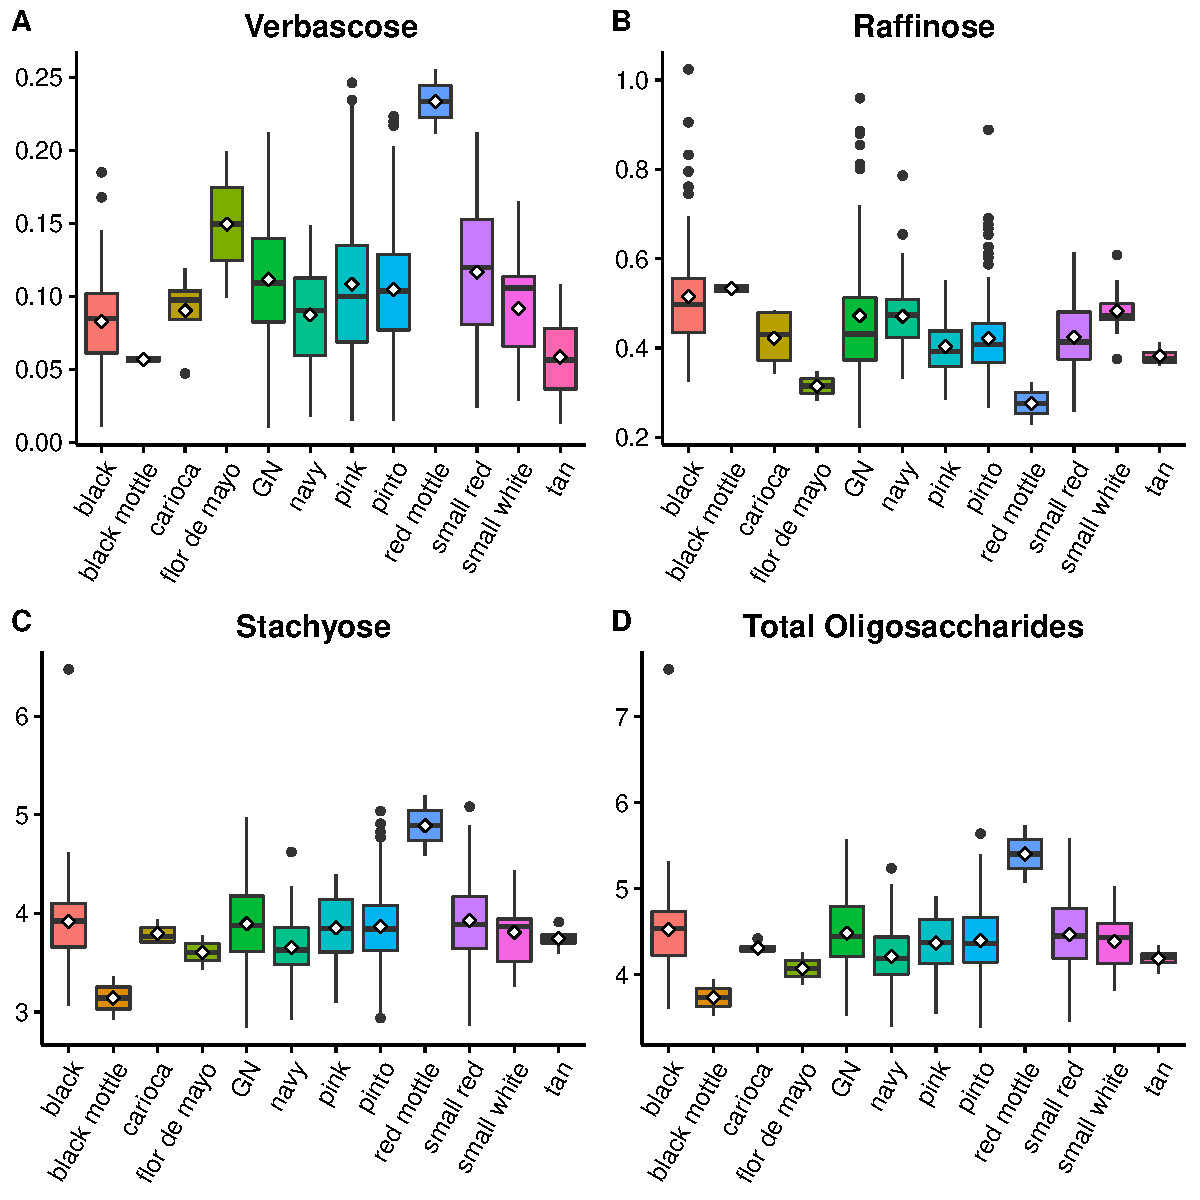
\includegraphics{./manuscript_template_files/figure-latex/unnamed-chunk-10-1} 

}

\caption{Oligosaccharide content in 282 common bean genotypes by marketclass (A) Raffinose, (B) Stachyose, (C) Verbascose, and (D) total oligosaccharides (= Raff + Stach + Verb).}\label{fig:unnamed-chunk-10}
\end{figure}

\begin{figure}

{\centering 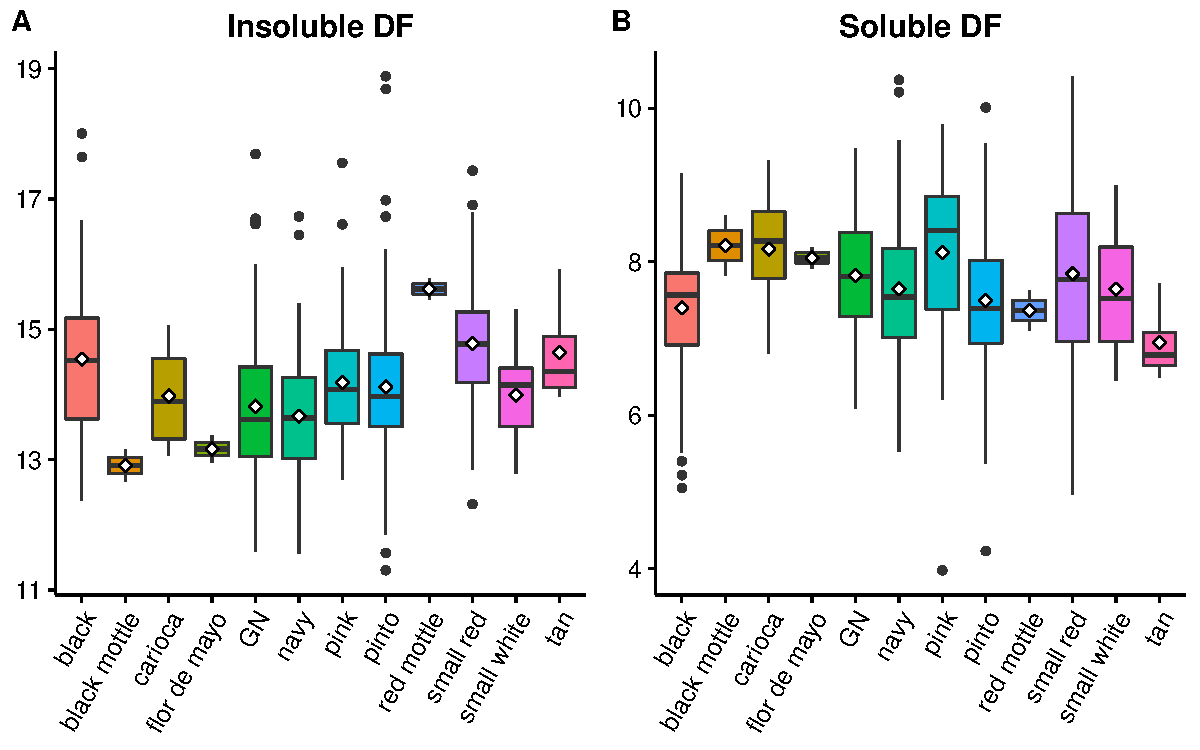
\includegraphics{./manuscript_template_files/figure-latex/unnamed-chunk-11-1} 

}

\caption{(A) Soluble and (B) insoluble dietary fiber in 282 common bean genotypes by marketclass,}\label{fig:unnamed-chunk-11}
\end{figure}

\begin{figure}

{\centering 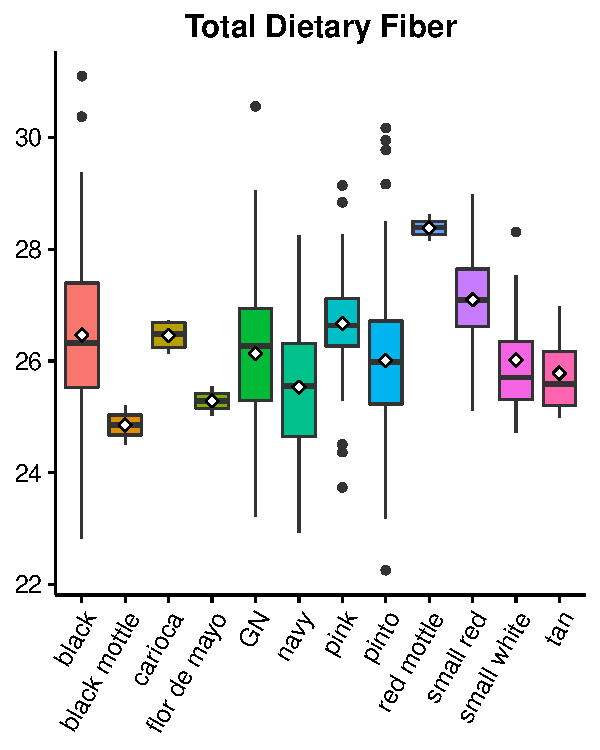
\includegraphics{./manuscript_template_files/figure-latex/unnamed-chunk-12-1} 

}

\caption{Total Dietary Fiber content in 282 common bean genotypes by marketclass}\label{fig:unnamed-chunk-12}
\end{figure}

\subsection{Results: Race}\label{results-race}

\begin{longtable}[c]{@{}lllllll@{}}
\toprule\addlinespace
Race & IDF & Verb & Raff & Stach & TOligos & TDF
\\\addlinespace
\midrule\endhead
Durango & 0.46a & 0.46a & 0.46a & 0.46a & 0.46a & 0.46a
\\\addlinespace
Jalisco & 0.03b
\\\addlinespace
Mesoamerican & 0.05a
\\\addlinespace
\bottomrule
\end{longtable}

\subsection{- Boxplots}\label{boxplots-1}

Figures below depict fiber content by race.

\begin{figure}

{\centering 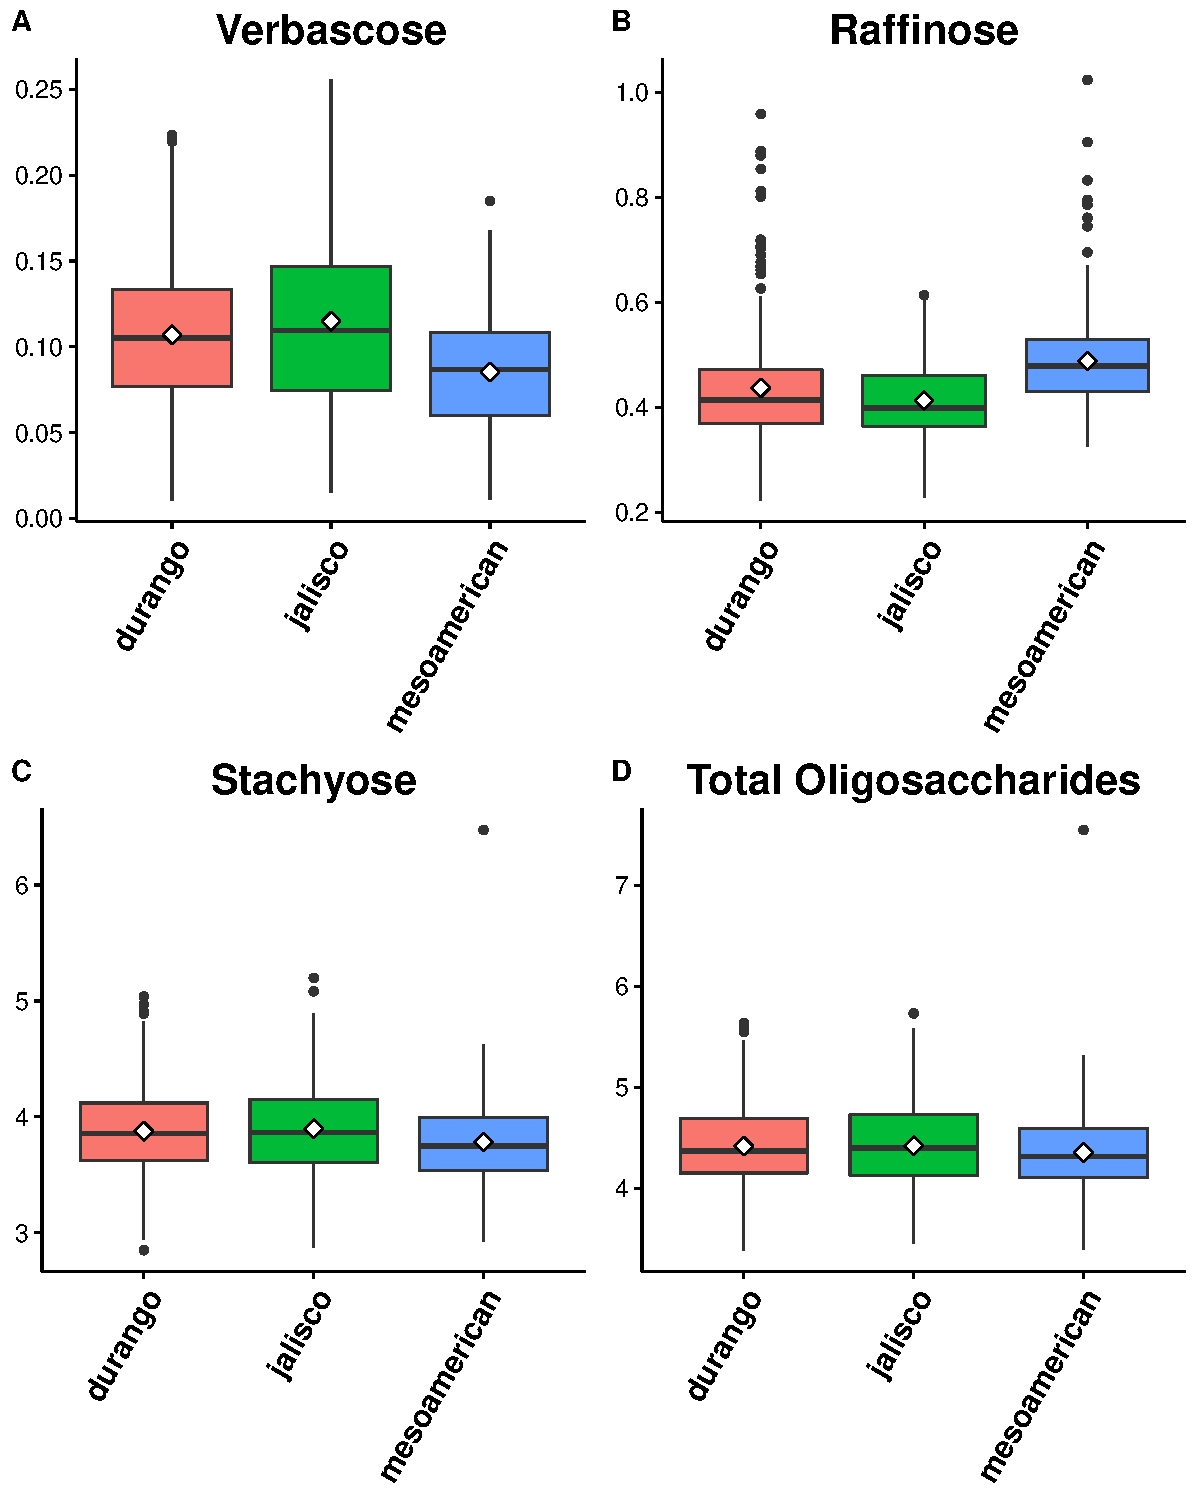
\includegraphics{./manuscript_template_files/figure-latex/unnamed-chunk-14-1} 

}

\caption{Oligosaccharide content in 282 common bean genotypes by race (A) Raffinose, (B) Stachyose, (C) Verbascose, and (D) total oligosaccharides (= Raff + Stach + Verb).}\label{fig:unnamed-chunk-14}
\end{figure}

\begin{figure}

{\centering 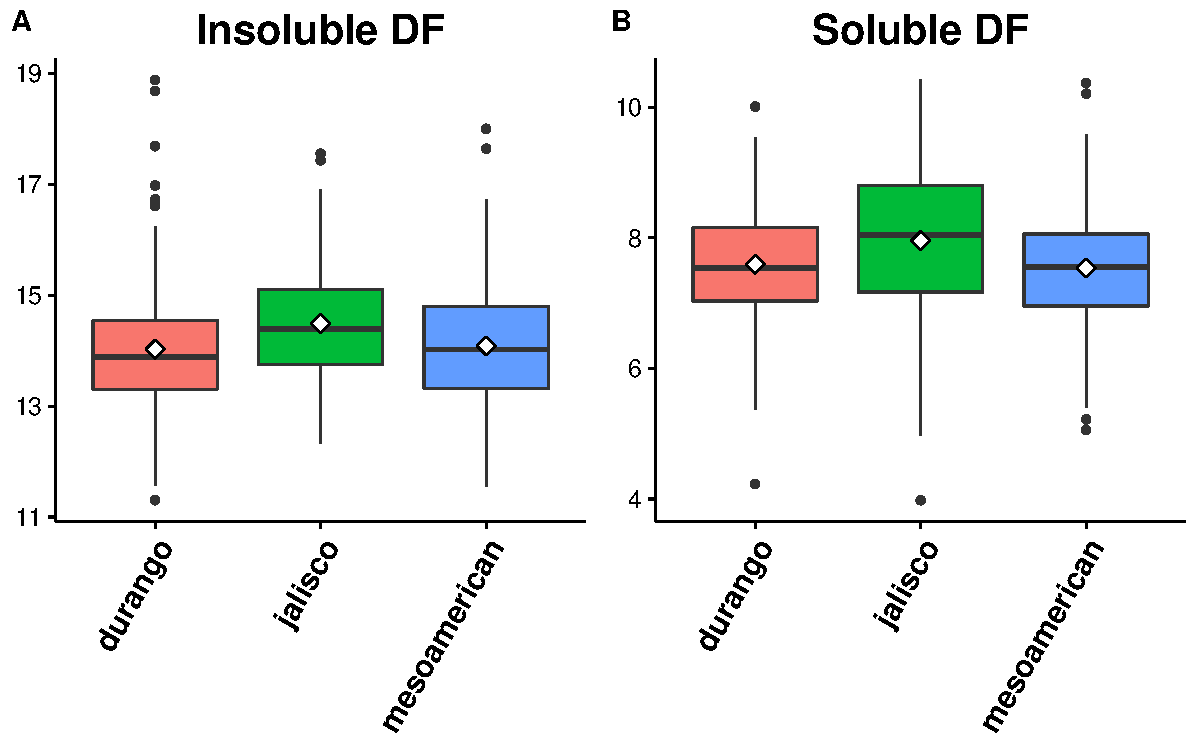
\includegraphics{./manuscript_template_files/figure-latex/unnamed-chunk-15-1} 

}

\caption{(A) Soluble and (B) insoluble dietary fiber in 282 common bean genotypes by race,}\label{fig:unnamed-chunk-15}
\end{figure}

\begin{figure}

{\centering 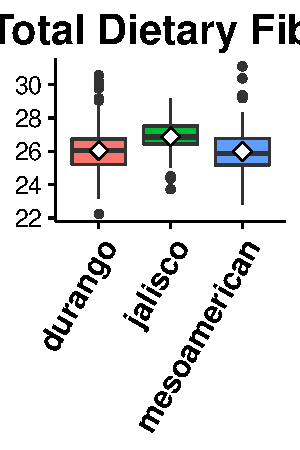
\includegraphics{./manuscript_template_files/figure-latex/unnamed-chunk-16-1} 

}

\caption{Total Dietary Fiber content in 282 common bean genotypes by race}\label{fig:unnamed-chunk-16}
\end{figure}
\newpage 
\end{document}